% Two ways to get the gradient back through a simulation, drawn as two vertical chains of states
% (a_0 at the top) for the backup slide, beside the memory plot (adjoint_memory.py).
% Compile: see ../build.sh (pdflatex, then pdftocairo -svg).
\documentclass[tikz,border=6pt]{standalone}
\usepackage{tikz}
\usepackage{amsmath}
\usepackage[T1]{fontenc}
\usetikzlibrary{arrows.meta,positioning,calc}

\definecolor{ink}{HTML}{2E2E2E}
\definecolor{greytx}{HTML}{6E6E6E}
\definecolor{fwd}{HTML}{3B6FB6}
\definecolor{revd}{HTML}{C0392B}
\definecolor{saved}{HTML}{2AA198}
\definecolor{panel}{HTML}{F4F6FA}

% #1 node-name tag, #2 x, #3 the stored states (a TikZ list)
\newcommand{\chain}[3]{%
  \foreach \i in {0,...,5}{%
    \node[draw=greytx,line width=1pt,fill=panel,rounded corners=4pt,
          minimum width=1.6cm,minimum height=0.95cm,text=ink,
          font=\sffamily\Large] (#1\i) at (#2,{-\i*1.55}) {$a_\i$};}
  \foreach \i in {0,...,4}{%
    \pgfmathtruncatemacro{\j}{\i+1}
    \draw[-{Stealth[length=5pt]},fwd,line width=1.4pt]
          (#1\i.west) to[bend right=50] (#1\j.west);
    \draw[-{Stealth[length=5pt]},revd,line width=1.4pt,densely dashed]
          (#1\j.east) to[bend right=50] (#1\i.east);}
  \foreach \i in #3{%
    \node[draw=saved,line width=2.4pt,rounded corners=4pt,
          minimum width=1.6cm,minimum height=0.95cm] at (#2,{-\i*1.55}) {};}}

\begin{document}
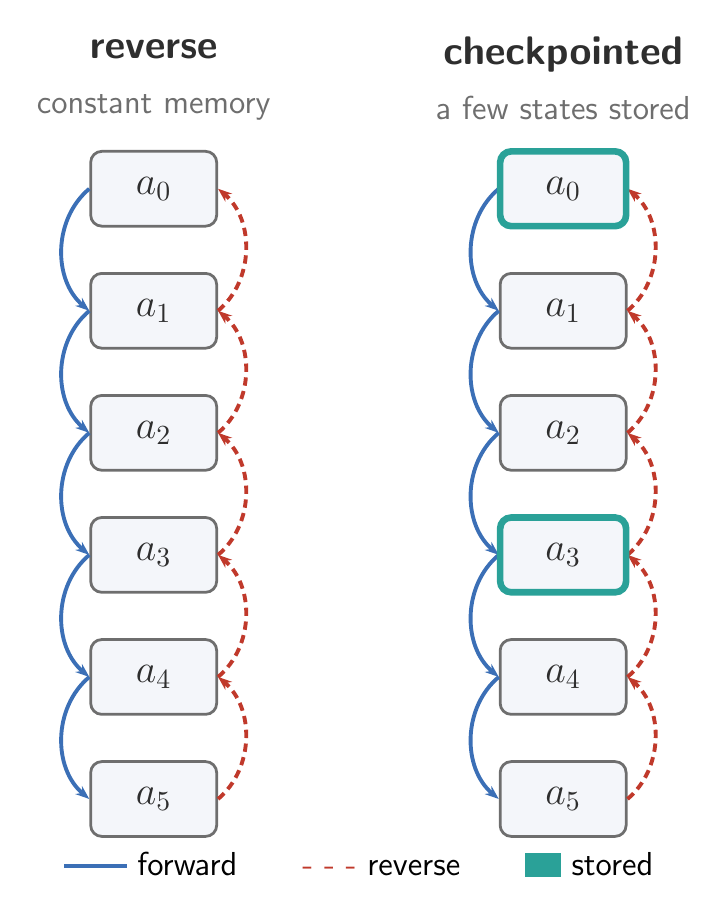
\begin{tikzpicture}[font=\sffamily]
  \chain{ra}{0}{{}}
  \chain{rb}{5.2}{{0,3}}
  \node[anchor=south,align=center,text=ink,font=\sffamily\Large] at (0,0.75)
       {\textbf{reverse}\\[2pt]\textcolor{greytx}{\large constant memory}};
  \node[anchor=south,align=center,text=ink,font=\sffamily\Large] at (5.2,0.75)
       {\textbf{checkpointed}\\[2pt]\textcolor{greytx}{\large a few states stored}};
  \node[anchor=north,align=left,font=\sffamily\large] at (2.6,-8.3)
       {\textcolor{fwd}{\rule[0.5ex]{0.8cm}{1.4pt}}\ forward\qquad
        \textcolor{revd}{- - -}\ reverse\qquad
        \textcolor{saved}{\rule[-0.1ex]{0.45cm}{0.3cm}}\ stored};
\end{tikzpicture}
\end{document}
